% Created by tikzDevice version 0.12 on 2019-06-13 16:13:07
% !TEX encoding = UTF-8 Unicode
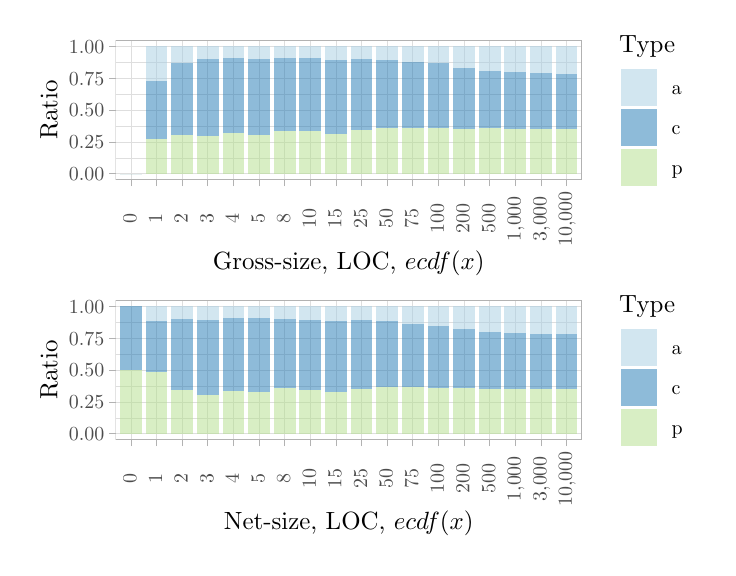
\begin{tikzpicture}[x=1pt,y=1pt]
\definecolor{fillColor}{RGB}{255,255,255}
\path[use as bounding box,fill=fillColor,fill opacity=0.00] (0,0) rectangle (245.72,187.90);
\begin{scope}
\path[clip] (  0.00, 93.95) rectangle (245.72,187.90);
\definecolor{drawColor}{RGB}{255,255,255}
\definecolor{fillColor}{RGB}{255,255,255}

\path[draw=drawColor,line width= 0.5pt,line join=round,line cap=round,fill=fillColor] (  0.00, 93.95) rectangle (245.72,187.90);
\end{scope}
\begin{scope}
\path[clip] ( 31.74,132.89) rectangle (200.26,183.40);
\definecolor{fillColor}{RGB}{255,255,255}

\path[fill=fillColor] ( 31.74,132.89) rectangle (200.26,183.40);
\definecolor{drawColor}{gray}{0.87}

\path[draw=drawColor,line width= 0.1pt,line join=round] ( 31.74,140.92) --
	(200.26,140.92);

\path[draw=drawColor,line width= 0.1pt,line join=round] ( 31.74,152.41) --
	(200.26,152.41);

\path[draw=drawColor,line width= 0.1pt,line join=round] ( 31.74,163.89) --
	(200.26,163.89);

\path[draw=drawColor,line width= 0.1pt,line join=round] ( 31.74,175.37) --
	(200.26,175.37);

\path[draw=drawColor,line width= 0.2pt,line join=round] ( 31.74,135.18) --
	(200.26,135.18);

\path[draw=drawColor,line width= 0.2pt,line join=round] ( 31.74,146.66) --
	(200.26,146.66);

\path[draw=drawColor,line width= 0.2pt,line join=round] ( 31.74,158.15) --
	(200.26,158.15);

\path[draw=drawColor,line width= 0.2pt,line join=round] ( 31.74,169.63) --
	(200.26,169.63);

\path[draw=drawColor,line width= 0.2pt,line join=round] ( 31.74,181.11) --
	(200.26,181.11);

\path[draw=drawColor,line width= 0.2pt,line join=round] ( 37.30,132.89) --
	( 37.30,183.40);

\path[draw=drawColor,line width= 0.2pt,line join=round] ( 46.55,132.89) --
	( 46.55,183.40);

\path[draw=drawColor,line width= 0.2pt,line join=round] ( 55.81,132.89) --
	( 55.81,183.40);

\path[draw=drawColor,line width= 0.2pt,line join=round] ( 65.07,132.89) --
	( 65.07,183.40);

\path[draw=drawColor,line width= 0.2pt,line join=round] ( 74.33,132.89) --
	( 74.33,183.40);

\path[draw=drawColor,line width= 0.2pt,line join=round] ( 83.59,132.89) --
	( 83.59,183.40);

\path[draw=drawColor,line width= 0.2pt,line join=round] ( 92.85,132.89) --
	( 92.85,183.40);

\path[draw=drawColor,line width= 0.2pt,line join=round] (102.11,132.89) --
	(102.11,183.40);

\path[draw=drawColor,line width= 0.2pt,line join=round] (111.37,132.89) --
	(111.37,183.40);

\path[draw=drawColor,line width= 0.2pt,line join=round] (120.63,132.89) --
	(120.63,183.40);

\path[draw=drawColor,line width= 0.2pt,line join=round] (129.89,132.89) --
	(129.89,183.40);

\path[draw=drawColor,line width= 0.2pt,line join=round] (139.15,132.89) --
	(139.15,183.40);

\path[draw=drawColor,line width= 0.2pt,line join=round] (148.41,132.89) --
	(148.41,183.40);

\path[draw=drawColor,line width= 0.2pt,line join=round] (157.67,132.89) --
	(157.67,183.40);

\path[draw=drawColor,line width= 0.2pt,line join=round] (166.93,132.89) --
	(166.93,183.40);

\path[draw=drawColor,line width= 0.2pt,line join=round] (176.19,132.89) --
	(176.19,183.40);

\path[draw=drawColor,line width= 0.2pt,line join=round] (185.45,132.89) --
	(185.45,183.40);

\path[draw=drawColor,line width= 0.2pt,line join=round] (194.71,132.89) --
	(194.71,183.40);
\definecolor{fillColor}{RGB}{178,223,138}

\path[fill=fillColor,fill opacity=0.50] ( 33.36,135.18) rectangle ( 41.23,135.18);
\definecolor{fillColor}{RGB}{31,120,180}

\path[fill=fillColor,fill opacity=0.50] ( 33.36,135.18) rectangle ( 41.23,135.18);
\definecolor{fillColor}{RGB}{166,206,227}

\path[fill=fillColor,fill opacity=0.50] ( 33.36,135.18) rectangle ( 41.23,135.18);
\definecolor{fillColor}{RGB}{178,223,138}

\path[fill=fillColor,fill opacity=0.50] ( 42.62,135.18) rectangle ( 50.49,147.71);
\definecolor{fillColor}{RGB}{31,120,180}

\path[fill=fillColor,fill opacity=0.50] ( 42.62,147.71) rectangle ( 50.49,168.58);
\definecolor{fillColor}{RGB}{166,206,227}

\path[fill=fillColor,fill opacity=0.50] ( 42.62,168.58) rectangle ( 50.49,181.11);
\definecolor{fillColor}{RGB}{178,223,138}

\path[fill=fillColor,fill opacity=0.50] ( 51.88,135.18) rectangle ( 59.75,149.16);
\definecolor{fillColor}{RGB}{31,120,180}

\path[fill=fillColor,fill opacity=0.50] ( 51.88,149.16) rectangle ( 59.75,175.12);
\definecolor{fillColor}{RGB}{166,206,227}

\path[fill=fillColor,fill opacity=0.50] ( 51.88,175.12) rectangle ( 59.75,181.11);
\definecolor{fillColor}{RGB}{178,223,138}

\path[fill=fillColor,fill opacity=0.50] ( 61.14,135.18) rectangle ( 69.01,148.75);
\definecolor{fillColor}{RGB}{31,120,180}

\path[fill=fillColor,fill opacity=0.50] ( 61.14,148.75) rectangle ( 69.01,176.41);
\definecolor{fillColor}{RGB}{166,206,227}

\path[fill=fillColor,fill opacity=0.50] ( 61.14,176.41) rectangle ( 69.01,181.11);
\definecolor{fillColor}{RGB}{178,223,138}

\path[fill=fillColor,fill opacity=0.50] ( 70.40,135.18) rectangle ( 78.27,149.67);
\definecolor{fillColor}{RGB}{31,120,180}

\path[fill=fillColor,fill opacity=0.50] ( 70.40,149.67) rectangle ( 78.27,176.87);
\definecolor{fillColor}{RGB}{166,206,227}

\path[fill=fillColor,fill opacity=0.50] ( 70.40,176.87) rectangle ( 78.27,181.11);
\definecolor{fillColor}{RGB}{178,223,138}

\path[fill=fillColor,fill opacity=0.50] ( 79.66,135.18) rectangle ( 87.53,149.08);
\definecolor{fillColor}{RGB}{31,120,180}

\path[fill=fillColor,fill opacity=0.50] ( 79.66,149.08) rectangle ( 87.53,176.57);
\definecolor{fillColor}{RGB}{166,206,227}

\path[fill=fillColor,fill opacity=0.50] ( 79.66,176.57) rectangle ( 87.53,181.11);
\definecolor{fillColor}{RGB}{178,223,138}

\path[fill=fillColor,fill opacity=0.50] ( 88.92,135.18) rectangle ( 96.79,150.42);
\definecolor{fillColor}{RGB}{31,120,180}

\path[fill=fillColor,fill opacity=0.50] ( 88.92,150.42) rectangle ( 96.79,176.93);
\definecolor{fillColor}{RGB}{166,206,227}

\path[fill=fillColor,fill opacity=0.50] ( 88.92,176.93) rectangle ( 96.79,181.11);
\definecolor{fillColor}{RGB}{178,223,138}

\path[fill=fillColor,fill opacity=0.50] ( 98.18,135.18) rectangle (106.05,150.49);
\definecolor{fillColor}{RGB}{31,120,180}

\path[fill=fillColor,fill opacity=0.50] ( 98.18,150.49) rectangle (106.05,176.88);
\definecolor{fillColor}{RGB}{166,206,227}

\path[fill=fillColor,fill opacity=0.50] ( 98.18,176.88) rectangle (106.05,181.11);
\definecolor{fillColor}{RGB}{178,223,138}

\path[fill=fillColor,fill opacity=0.50] (107.44,135.18) rectangle (115.31,149.59);
\definecolor{fillColor}{RGB}{31,120,180}

\path[fill=fillColor,fill opacity=0.50] (107.44,149.59) rectangle (115.31,176.12);
\definecolor{fillColor}{RGB}{166,206,227}

\path[fill=fillColor,fill opacity=0.50] (107.44,176.12) rectangle (115.31,181.11);
\definecolor{fillColor}{RGB}{178,223,138}

\path[fill=fillColor,fill opacity=0.50] (116.70,135.18) rectangle (124.57,150.87);
\definecolor{fillColor}{RGB}{31,120,180}

\path[fill=fillColor,fill opacity=0.50] (116.70,150.87) rectangle (124.57,176.53);
\definecolor{fillColor}{RGB}{166,206,227}

\path[fill=fillColor,fill opacity=0.50] (116.70,176.53) rectangle (124.57,181.11);
\definecolor{fillColor}{RGB}{178,223,138}

\path[fill=fillColor,fill opacity=0.50] (125.96,135.18) rectangle (133.83,151.61);
\definecolor{fillColor}{RGB}{31,120,180}

\path[fill=fillColor,fill opacity=0.50] (125.96,151.61) rectangle (133.83,176.24);
\definecolor{fillColor}{RGB}{166,206,227}

\path[fill=fillColor,fill opacity=0.50] (125.96,176.24) rectangle (133.83,181.11);
\definecolor{fillColor}{RGB}{178,223,138}

\path[fill=fillColor,fill opacity=0.50] (135.22,135.18) rectangle (143.09,151.65);
\definecolor{fillColor}{RGB}{31,120,180}

\path[fill=fillColor,fill opacity=0.50] (135.22,151.65) rectangle (143.09,175.36);
\definecolor{fillColor}{RGB}{166,206,227}

\path[fill=fillColor,fill opacity=0.50] (135.22,175.36) rectangle (143.09,181.11);
\definecolor{fillColor}{RGB}{178,223,138}

\path[fill=fillColor,fill opacity=0.50] (144.48,135.18) rectangle (152.35,151.73);
\definecolor{fillColor}{RGB}{31,120,180}

\path[fill=fillColor,fill opacity=0.50] (144.48,151.73) rectangle (152.35,174.96);
\definecolor{fillColor}{RGB}{166,206,227}

\path[fill=fillColor,fill opacity=0.50] (144.48,174.96) rectangle (152.35,181.11);
\definecolor{fillColor}{RGB}{178,223,138}

\path[fill=fillColor,fill opacity=0.50] (153.74,135.18) rectangle (161.61,151.44);
\definecolor{fillColor}{RGB}{31,120,180}

\path[fill=fillColor,fill opacity=0.50] (153.74,151.44) rectangle (161.61,173.43);
\definecolor{fillColor}{RGB}{166,206,227}

\path[fill=fillColor,fill opacity=0.50] (153.74,173.43) rectangle (161.61,181.11);
\definecolor{fillColor}{RGB}{178,223,138}

\path[fill=fillColor,fill opacity=0.50] (162.99,135.18) rectangle (170.87,151.48);
\definecolor{fillColor}{RGB}{31,120,180}

\path[fill=fillColor,fill opacity=0.50] (162.99,151.48) rectangle (170.87,172.42);
\definecolor{fillColor}{RGB}{166,206,227}

\path[fill=fillColor,fill opacity=0.50] (162.99,172.42) rectangle (170.87,181.11);
\definecolor{fillColor}{RGB}{178,223,138}

\path[fill=fillColor,fill opacity=0.50] (172.25,135.18) rectangle (180.13,151.37);
\definecolor{fillColor}{RGB}{31,120,180}

\path[fill=fillColor,fill opacity=0.50] (172.25,151.37) rectangle (180.13,171.79);
\definecolor{fillColor}{RGB}{166,206,227}

\path[fill=fillColor,fill opacity=0.50] (172.25,171.79) rectangle (180.13,181.11);
\definecolor{fillColor}{RGB}{178,223,138}

\path[fill=fillColor,fill opacity=0.50] (181.51,135.18) rectangle (189.38,151.30);
\definecolor{fillColor}{RGB}{31,120,180}

\path[fill=fillColor,fill opacity=0.50] (181.51,151.30) rectangle (189.38,171.41);
\definecolor{fillColor}{RGB}{166,206,227}

\path[fill=fillColor,fill opacity=0.50] (181.51,171.41) rectangle (189.38,181.11);
\definecolor{fillColor}{RGB}{178,223,138}

\path[fill=fillColor,fill opacity=0.50] (190.77,135.18) rectangle (198.64,151.28);
\definecolor{fillColor}{RGB}{31,120,180}

\path[fill=fillColor,fill opacity=0.50] (190.77,151.28) rectangle (198.64,171.26);
\definecolor{fillColor}{RGB}{166,206,227}

\path[fill=fillColor,fill opacity=0.50] (190.77,171.26) rectangle (198.64,181.11);
\definecolor{drawColor}{gray}{0.70}

\path[draw=drawColor,line width= 0.5pt,line join=round,line cap=round] ( 31.74,132.89) rectangle (200.26,183.40);
\end{scope}
\begin{scope}
\path[clip] (  0.00,  0.00) rectangle (245.72,187.90);
\definecolor{drawColor}{gray}{0.30}

\node[text=drawColor,anchor=base east,inner sep=0pt, outer sep=0pt, scale=  0.72] at ( 27.69,132.71) {0.00};

\node[text=drawColor,anchor=base east,inner sep=0pt, outer sep=0pt, scale=  0.72] at ( 27.69,144.19) {0.25};

\node[text=drawColor,anchor=base east,inner sep=0pt, outer sep=0pt, scale=  0.72] at ( 27.69,155.67) {0.50};

\node[text=drawColor,anchor=base east,inner sep=0pt, outer sep=0pt, scale=  0.72] at ( 27.69,167.15) {0.75};

\node[text=drawColor,anchor=base east,inner sep=0pt, outer sep=0pt, scale=  0.72] at ( 27.69,178.63) {1.00};
\end{scope}
\begin{scope}
\path[clip] (  0.00,  0.00) rectangle (245.72,187.90);
\definecolor{drawColor}{gray}{0.70}

\path[draw=drawColor,line width= 0.2pt,line join=round] ( 29.49,135.18) --
	( 31.74,135.18);

\path[draw=drawColor,line width= 0.2pt,line join=round] ( 29.49,146.66) --
	( 31.74,146.66);

\path[draw=drawColor,line width= 0.2pt,line join=round] ( 29.49,158.15) --
	( 31.74,158.15);

\path[draw=drawColor,line width= 0.2pt,line join=round] ( 29.49,169.63) --
	( 31.74,169.63);

\path[draw=drawColor,line width= 0.2pt,line join=round] ( 29.49,181.11) --
	( 31.74,181.11);
\end{scope}
\begin{scope}
\path[clip] (  0.00,  0.00) rectangle (245.72,187.90);
\definecolor{drawColor}{gray}{0.70}

\path[draw=drawColor,line width= 0.2pt,line join=round] ( 37.30,130.64) --
	( 37.30,132.89);

\path[draw=drawColor,line width= 0.2pt,line join=round] ( 46.55,130.64) --
	( 46.55,132.89);

\path[draw=drawColor,line width= 0.2pt,line join=round] ( 55.81,130.64) --
	( 55.81,132.89);

\path[draw=drawColor,line width= 0.2pt,line join=round] ( 65.07,130.64) --
	( 65.07,132.89);

\path[draw=drawColor,line width= 0.2pt,line join=round] ( 74.33,130.64) --
	( 74.33,132.89);

\path[draw=drawColor,line width= 0.2pt,line join=round] ( 83.59,130.64) --
	( 83.59,132.89);

\path[draw=drawColor,line width= 0.2pt,line join=round] ( 92.85,130.64) --
	( 92.85,132.89);

\path[draw=drawColor,line width= 0.2pt,line join=round] (102.11,130.64) --
	(102.11,132.89);

\path[draw=drawColor,line width= 0.2pt,line join=round] (111.37,130.64) --
	(111.37,132.89);

\path[draw=drawColor,line width= 0.2pt,line join=round] (120.63,130.64) --
	(120.63,132.89);

\path[draw=drawColor,line width= 0.2pt,line join=round] (129.89,130.64) --
	(129.89,132.89);

\path[draw=drawColor,line width= 0.2pt,line join=round] (139.15,130.64) --
	(139.15,132.89);

\path[draw=drawColor,line width= 0.2pt,line join=round] (148.41,130.64) --
	(148.41,132.89);

\path[draw=drawColor,line width= 0.2pt,line join=round] (157.67,130.64) --
	(157.67,132.89);

\path[draw=drawColor,line width= 0.2pt,line join=round] (166.93,130.64) --
	(166.93,132.89);

\path[draw=drawColor,line width= 0.2pt,line join=round] (176.19,130.64) --
	(176.19,132.89);

\path[draw=drawColor,line width= 0.2pt,line join=round] (185.45,130.64) --
	(185.45,132.89);

\path[draw=drawColor,line width= 0.2pt,line join=round] (194.71,130.64) --
	(194.71,132.89);
\end{scope}
\begin{scope}
\path[clip] (  0.00,  0.00) rectangle (245.72,187.90);
\definecolor{drawColor}{gray}{0.30}

\node[text=drawColor,rotate= 90.00,anchor=base,inner sep=0pt, outer sep=0pt, scale=  0.72] at ( 39.28,118.84) {     0};

\node[text=drawColor,rotate= 90.00,anchor=base,inner sep=0pt, outer sep=0pt, scale=  0.72] at ( 48.54,118.84) {     1};

\node[text=drawColor,rotate= 90.00,anchor=base,inner sep=0pt, outer sep=0pt, scale=  0.72] at ( 57.80,118.84) {     2};

\node[text=drawColor,rotate= 90.00,anchor=base,inner sep=0pt, outer sep=0pt, scale=  0.72] at ( 67.06,118.84) {     3};

\node[text=drawColor,rotate= 90.00,anchor=base,inner sep=0pt, outer sep=0pt, scale=  0.72] at ( 76.32,118.84) {     4};

\node[text=drawColor,rotate= 90.00,anchor=base,inner sep=0pt, outer sep=0pt, scale=  0.72] at ( 85.58,118.84) {     5};

\node[text=drawColor,rotate= 90.00,anchor=base,inner sep=0pt, outer sep=0pt, scale=  0.72] at ( 94.84,118.84) {     8};

\node[text=drawColor,rotate= 90.00,anchor=base,inner sep=0pt, outer sep=0pt, scale=  0.72] at (104.10,118.84) {    10};

\node[text=drawColor,rotate= 90.00,anchor=base,inner sep=0pt, outer sep=0pt, scale=  0.72] at (113.36,118.84) {    15};

\node[text=drawColor,rotate= 90.00,anchor=base,inner sep=0pt, outer sep=0pt, scale=  0.72] at (122.62,118.84) {    25};

\node[text=drawColor,rotate= 90.00,anchor=base,inner sep=0pt, outer sep=0pt, scale=  0.72] at (131.88,118.84) {    50};

\node[text=drawColor,rotate= 90.00,anchor=base,inner sep=0pt, outer sep=0pt, scale=  0.72] at (141.13,118.84) {    75};

\node[text=drawColor,rotate= 90.00,anchor=base,inner sep=0pt, outer sep=0pt, scale=  0.72] at (150.39,118.84) {   100};

\node[text=drawColor,rotate= 90.00,anchor=base,inner sep=0pt, outer sep=0pt, scale=  0.72] at (159.65,118.84) {   200};

\node[text=drawColor,rotate= 90.00,anchor=base,inner sep=0pt, outer sep=0pt, scale=  0.72] at (168.91,118.84) {   500};

\node[text=drawColor,rotate= 90.00,anchor=base,inner sep=0pt, outer sep=0pt, scale=  0.72] at (178.17,118.84) { 1,000};

\node[text=drawColor,rotate= 90.00,anchor=base,inner sep=0pt, outer sep=0pt, scale=  0.72] at (187.43,118.84) { 3,000};

\node[text=drawColor,rotate= 90.00,anchor=base,inner sep=0pt, outer sep=0pt, scale=  0.72] at (196.69,118.84) {10,000};
\end{scope}
\begin{scope}
\path[clip] (  0.00,  0.00) rectangle (245.72,187.90);
\definecolor{drawColor}{RGB}{0,0,0}

\node[text=drawColor,anchor=base,inner sep=0pt, outer sep=0pt, scale=  0.90] at (116.00,100.39) {Gross-size, LOC, $ecdf(x)$};
\end{scope}
\begin{scope}
\path[clip] (  0.00,  0.00) rectangle (245.72,187.90);
\definecolor{drawColor}{RGB}{0,0,0}

\node[text=drawColor,rotate= 90.00,anchor=base,inner sep=0pt, outer sep=0pt, scale=  0.90] at ( 10.70,158.15) {Ratio};
\end{scope}
\begin{scope}
\path[clip] (  0.00,  0.00) rectangle (245.72,187.90);
\definecolor{fillColor}{RGB}{255,255,255}

\path[fill=fillColor] (209.26,125.64) rectangle (241.22,190.65);
\end{scope}
\begin{scope}
\path[clip] (  0.00,  0.00) rectangle (245.72,187.90);
\definecolor{drawColor}{RGB}{0,0,0}

\node[text=drawColor,anchor=base west,inner sep=0pt, outer sep=0pt, scale=  0.90] at (213.76,178.98) {Type};
\end{scope}
\begin{scope}
\path[clip] (  0.00,  0.00) rectangle (245.72,187.90);
\definecolor{fillColor}{RGB}{255,255,255}

\path[fill=fillColor] (213.76,159.05) rectangle (228.22,173.51);
\end{scope}
\begin{scope}
\path[clip] (  0.00,  0.00) rectangle (245.72,187.90);
\definecolor{fillColor}{RGB}{166,206,227}

\path[fill=fillColor,fill opacity=0.50] (214.48,159.76) rectangle (227.51,172.79);
\end{scope}
\begin{scope}
\path[clip] (  0.00,  0.00) rectangle (245.72,187.90);
\definecolor{fillColor}{RGB}{255,255,255}

\path[fill=fillColor] (213.76,144.60) rectangle (228.22,159.05);
\end{scope}
\begin{scope}
\path[clip] (  0.00,  0.00) rectangle (245.72,187.90);
\definecolor{fillColor}{RGB}{31,120,180}

\path[fill=fillColor,fill opacity=0.50] (214.48,145.31) rectangle (227.51,158.34);
\end{scope}
\begin{scope}
\path[clip] (  0.00,  0.00) rectangle (245.72,187.90);
\definecolor{fillColor}{RGB}{255,255,255}

\path[fill=fillColor] (213.76,130.14) rectangle (228.22,144.60);
\end{scope}
\begin{scope}
\path[clip] (  0.00,  0.00) rectangle (245.72,187.90);
\definecolor{fillColor}{RGB}{178,223,138}

\path[fill=fillColor,fill opacity=0.50] (214.48,130.85) rectangle (227.51,143.89);
\end{scope}
\begin{scope}
\path[clip] (  0.00,  0.00) rectangle (245.72,187.90);
\definecolor{drawColor}{RGB}{0,0,0}

\node[text=drawColor,anchor=base west,inner sep=0pt, outer sep=0pt, scale=  0.72] at (232.72,163.80) {a};
\end{scope}
\begin{scope}
\path[clip] (  0.00,  0.00) rectangle (245.72,187.90);
\definecolor{drawColor}{RGB}{0,0,0}

\node[text=drawColor,anchor=base west,inner sep=0pt, outer sep=0pt, scale=  0.72] at (232.72,149.34) {c};
\end{scope}
\begin{scope}
\path[clip] (  0.00,  0.00) rectangle (245.72,187.90);
\definecolor{drawColor}{RGB}{0,0,0}

\node[text=drawColor,anchor=base west,inner sep=0pt, outer sep=0pt, scale=  0.72] at (232.72,134.89) {p};
\end{scope}
\begin{scope}
\path[clip] (  0.00,  0.00) rectangle (245.72, 93.95);
\definecolor{drawColor}{RGB}{255,255,255}
\definecolor{fillColor}{RGB}{255,255,255}

\path[draw=drawColor,line width= 0.5pt,line join=round,line cap=round,fill=fillColor] (  0.00,  0.00) rectangle (245.72, 93.95);
\end{scope}
\begin{scope}
\path[clip] ( 31.74, 38.94) rectangle (200.26, 89.45);
\definecolor{fillColor}{RGB}{255,255,255}

\path[fill=fillColor] ( 31.74, 38.94) rectangle (200.26, 89.45);
\definecolor{drawColor}{gray}{0.87}

\path[draw=drawColor,line width= 0.1pt,line join=round] ( 31.74, 46.97) --
	(200.26, 46.97);

\path[draw=drawColor,line width= 0.1pt,line join=round] ( 31.74, 58.45) --
	(200.26, 58.45);

\path[draw=drawColor,line width= 0.1pt,line join=round] ( 31.74, 69.93) --
	(200.26, 69.93);

\path[draw=drawColor,line width= 0.1pt,line join=round] ( 31.74, 81.41) --
	(200.26, 81.41);

\path[draw=drawColor,line width= 0.2pt,line join=round] ( 31.74, 41.23) --
	(200.26, 41.23);

\path[draw=drawColor,line width= 0.2pt,line join=round] ( 31.74, 52.71) --
	(200.26, 52.71);

\path[draw=drawColor,line width= 0.2pt,line join=round] ( 31.74, 64.19) --
	(200.26, 64.19);

\path[draw=drawColor,line width= 0.2pt,line join=round] ( 31.74, 75.67) --
	(200.26, 75.67);

\path[draw=drawColor,line width= 0.2pt,line join=round] ( 31.74, 87.15) --
	(200.26, 87.15);

\path[draw=drawColor,line width= 0.2pt,line join=round] ( 37.30, 38.94) --
	( 37.30, 89.45);

\path[draw=drawColor,line width= 0.2pt,line join=round] ( 46.55, 38.94) --
	( 46.55, 89.45);

\path[draw=drawColor,line width= 0.2pt,line join=round] ( 55.81, 38.94) --
	( 55.81, 89.45);

\path[draw=drawColor,line width= 0.2pt,line join=round] ( 65.07, 38.94) --
	( 65.07, 89.45);

\path[draw=drawColor,line width= 0.2pt,line join=round] ( 74.33, 38.94) --
	( 74.33, 89.45);

\path[draw=drawColor,line width= 0.2pt,line join=round] ( 83.59, 38.94) --
	( 83.59, 89.45);

\path[draw=drawColor,line width= 0.2pt,line join=round] ( 92.85, 38.94) --
	( 92.85, 89.45);

\path[draw=drawColor,line width= 0.2pt,line join=round] (102.11, 38.94) --
	(102.11, 89.45);

\path[draw=drawColor,line width= 0.2pt,line join=round] (111.37, 38.94) --
	(111.37, 89.45);

\path[draw=drawColor,line width= 0.2pt,line join=round] (120.63, 38.94) --
	(120.63, 89.45);

\path[draw=drawColor,line width= 0.2pt,line join=round] (129.89, 38.94) --
	(129.89, 89.45);

\path[draw=drawColor,line width= 0.2pt,line join=round] (139.15, 38.94) --
	(139.15, 89.45);

\path[draw=drawColor,line width= 0.2pt,line join=round] (148.41, 38.94) --
	(148.41, 89.45);

\path[draw=drawColor,line width= 0.2pt,line join=round] (157.67, 38.94) --
	(157.67, 89.45);

\path[draw=drawColor,line width= 0.2pt,line join=round] (166.93, 38.94) --
	(166.93, 89.45);

\path[draw=drawColor,line width= 0.2pt,line join=round] (176.19, 38.94) --
	(176.19, 89.45);

\path[draw=drawColor,line width= 0.2pt,line join=round] (185.45, 38.94) --
	(185.45, 89.45);

\path[draw=drawColor,line width= 0.2pt,line join=round] (194.71, 38.94) --
	(194.71, 89.45);
\definecolor{fillColor}{RGB}{178,223,138}

\path[fill=fillColor,fill opacity=0.50] ( 33.36, 41.23) rectangle ( 41.23, 64.19);
\definecolor{fillColor}{RGB}{31,120,180}

\path[fill=fillColor,fill opacity=0.50] ( 33.36, 64.19) rectangle ( 41.23, 87.15);
\definecolor{fillColor}{RGB}{166,206,227}

\path[fill=fillColor,fill opacity=0.50] ( 33.36, 87.15) rectangle ( 41.23, 87.15);
\definecolor{fillColor}{RGB}{178,223,138}

\path[fill=fillColor,fill opacity=0.50] ( 42.62, 41.23) rectangle ( 50.49, 63.34);
\definecolor{fillColor}{RGB}{31,120,180}

\path[fill=fillColor,fill opacity=0.50] ( 42.62, 63.34) rectangle ( 50.49, 82.05);
\definecolor{fillColor}{RGB}{166,206,227}

\path[fill=fillColor,fill opacity=0.50] ( 42.62, 82.05) rectangle ( 50.49, 87.15);
\definecolor{fillColor}{RGB}{178,223,138}

\path[fill=fillColor,fill opacity=0.50] ( 51.88, 41.23) rectangle ( 59.75, 57.05);
\definecolor{fillColor}{RGB}{31,120,180}

\path[fill=fillColor,fill opacity=0.50] ( 51.88, 57.05) rectangle ( 59.75, 82.56);
\definecolor{fillColor}{RGB}{166,206,227}

\path[fill=fillColor,fill opacity=0.50] ( 51.88, 82.56) rectangle ( 59.75, 87.15);
\definecolor{fillColor}{RGB}{178,223,138}

\path[fill=fillColor,fill opacity=0.50] ( 61.14, 41.23) rectangle ( 69.01, 55.24);
\definecolor{fillColor}{RGB}{31,120,180}

\path[fill=fillColor,fill opacity=0.50] ( 61.14, 55.24) rectangle ( 69.01, 82.10);
\definecolor{fillColor}{RGB}{166,206,227}

\path[fill=fillColor,fill opacity=0.50] ( 61.14, 82.10) rectangle ( 69.01, 87.15);
\definecolor{fillColor}{RGB}{178,223,138}

\path[fill=fillColor,fill opacity=0.50] ( 70.40, 41.23) rectangle ( 78.27, 56.54);
\definecolor{fillColor}{RGB}{31,120,180}

\path[fill=fillColor,fill opacity=0.50] ( 70.40, 56.54) rectangle ( 78.27, 82.90);
\definecolor{fillColor}{RGB}{166,206,227}

\path[fill=fillColor,fill opacity=0.50] ( 70.40, 82.90) rectangle ( 78.27, 87.15);
\definecolor{fillColor}{RGB}{178,223,138}

\path[fill=fillColor,fill opacity=0.50] ( 79.66, 41.23) rectangle ( 87.53, 56.29);
\definecolor{fillColor}{RGB}{31,120,180}

\path[fill=fillColor,fill opacity=0.50] ( 79.66, 56.29) rectangle ( 87.53, 83.07);
\definecolor{fillColor}{RGB}{166,206,227}

\path[fill=fillColor,fill opacity=0.50] ( 79.66, 83.07) rectangle ( 87.53, 87.15);
\definecolor{fillColor}{RGB}{178,223,138}

\path[fill=fillColor,fill opacity=0.50] ( 88.92, 41.23) rectangle ( 96.79, 57.62);
\definecolor{fillColor}{RGB}{31,120,180}

\path[fill=fillColor,fill opacity=0.50] ( 88.92, 57.62) rectangle ( 96.79, 82.65);
\definecolor{fillColor}{RGB}{166,206,227}

\path[fill=fillColor,fill opacity=0.50] ( 88.92, 82.65) rectangle ( 96.79, 87.15);
\definecolor{fillColor}{RGB}{178,223,138}

\path[fill=fillColor,fill opacity=0.50] ( 98.18, 41.23) rectangle (106.05, 56.94);
\definecolor{fillColor}{RGB}{31,120,180}

\path[fill=fillColor,fill opacity=0.50] ( 98.18, 56.94) rectangle (106.05, 82.32);
\definecolor{fillColor}{RGB}{166,206,227}

\path[fill=fillColor,fill opacity=0.50] ( 98.18, 82.32) rectangle (106.05, 87.15);
\definecolor{fillColor}{RGB}{178,223,138}

\path[fill=fillColor,fill opacity=0.50] (107.44, 41.23) rectangle (115.31, 56.34);
\definecolor{fillColor}{RGB}{31,120,180}

\path[fill=fillColor,fill opacity=0.50] (107.44, 56.34) rectangle (115.31, 82.04);
\definecolor{fillColor}{RGB}{166,206,227}

\path[fill=fillColor,fill opacity=0.50] (107.44, 82.04) rectangle (115.31, 87.15);
\definecolor{fillColor}{RGB}{178,223,138}

\path[fill=fillColor,fill opacity=0.50] (116.70, 41.23) rectangle (124.57, 57.21);
\definecolor{fillColor}{RGB}{31,120,180}

\path[fill=fillColor,fill opacity=0.50] (116.70, 57.21) rectangle (124.57, 82.25);
\definecolor{fillColor}{RGB}{166,206,227}

\path[fill=fillColor,fill opacity=0.50] (116.70, 82.25) rectangle (124.57, 87.15);
\definecolor{fillColor}{RGB}{178,223,138}

\path[fill=fillColor,fill opacity=0.50] (125.96, 41.23) rectangle (133.83, 57.98);
\definecolor{fillColor}{RGB}{31,120,180}

\path[fill=fillColor,fill opacity=0.50] (125.96, 57.98) rectangle (133.83, 81.73);
\definecolor{fillColor}{RGB}{166,206,227}

\path[fill=fillColor,fill opacity=0.50] (125.96, 81.73) rectangle (133.83, 87.15);
\definecolor{fillColor}{RGB}{178,223,138}

\path[fill=fillColor,fill opacity=0.50] (135.22, 41.23) rectangle (143.09, 58.01);
\definecolor{fillColor}{RGB}{31,120,180}

\path[fill=fillColor,fill opacity=0.50] (135.22, 58.01) rectangle (143.09, 80.74);
\definecolor{fillColor}{RGB}{166,206,227}

\path[fill=fillColor,fill opacity=0.50] (135.22, 80.74) rectangle (143.09, 87.15);
\definecolor{fillColor}{RGB}{178,223,138}

\path[fill=fillColor,fill opacity=0.50] (144.48, 41.23) rectangle (152.35, 57.85);
\definecolor{fillColor}{RGB}{31,120,180}

\path[fill=fillColor,fill opacity=0.50] (144.48, 57.85) rectangle (152.35, 80.16);
\definecolor{fillColor}{RGB}{166,206,227}

\path[fill=fillColor,fill opacity=0.50] (144.48, 80.16) rectangle (152.35, 87.15);
\definecolor{fillColor}{RGB}{178,223,138}

\path[fill=fillColor,fill opacity=0.50] (153.74, 41.23) rectangle (161.61, 57.79);
\definecolor{fillColor}{RGB}{31,120,180}

\path[fill=fillColor,fill opacity=0.50] (153.74, 57.79) rectangle (161.61, 78.95);
\definecolor{fillColor}{RGB}{166,206,227}

\path[fill=fillColor,fill opacity=0.50] (153.74, 78.95) rectangle (161.61, 87.15);
\definecolor{fillColor}{RGB}{178,223,138}

\path[fill=fillColor,fill opacity=0.50] (162.99, 41.23) rectangle (170.87, 57.42);
\definecolor{fillColor}{RGB}{31,120,180}

\path[fill=fillColor,fill opacity=0.50] (162.99, 57.42) rectangle (170.87, 78.11);
\definecolor{fillColor}{RGB}{166,206,227}

\path[fill=fillColor,fill opacity=0.50] (162.99, 78.11) rectangle (170.87, 87.15);
\definecolor{fillColor}{RGB}{178,223,138}

\path[fill=fillColor,fill opacity=0.50] (172.25, 41.23) rectangle (180.13, 57.44);
\definecolor{fillColor}{RGB}{31,120,180}

\path[fill=fillColor,fill opacity=0.50] (172.25, 57.44) rectangle (180.13, 77.68);
\definecolor{fillColor}{RGB}{166,206,227}

\path[fill=fillColor,fill opacity=0.50] (172.25, 77.68) rectangle (180.13, 87.15);
\definecolor{fillColor}{RGB}{178,223,138}

\path[fill=fillColor,fill opacity=0.50] (181.51, 41.23) rectangle (189.38, 57.37);
\definecolor{fillColor}{RGB}{31,120,180}

\path[fill=fillColor,fill opacity=0.50] (181.51, 57.37) rectangle (189.38, 77.36);
\definecolor{fillColor}{RGB}{166,206,227}

\path[fill=fillColor,fill opacity=0.50] (181.51, 77.36) rectangle (189.38, 87.15);
\definecolor{fillColor}{RGB}{178,223,138}

\path[fill=fillColor,fill opacity=0.50] (190.77, 41.23) rectangle (198.64, 57.31);
\definecolor{fillColor}{RGB}{31,120,180}

\path[fill=fillColor,fill opacity=0.50] (190.77, 57.31) rectangle (198.64, 77.31);
\definecolor{fillColor}{RGB}{166,206,227}

\path[fill=fillColor,fill opacity=0.50] (190.77, 77.31) rectangle (198.64, 87.15);
\definecolor{drawColor}{gray}{0.70}

\path[draw=drawColor,line width= 0.5pt,line join=round,line cap=round] ( 31.74, 38.94) rectangle (200.26, 89.45);
\end{scope}
\begin{scope}
\path[clip] (  0.00,  0.00) rectangle (245.72,187.90);
\definecolor{drawColor}{gray}{0.30}

\node[text=drawColor,anchor=base east,inner sep=0pt, outer sep=0pt, scale=  0.72] at ( 27.69, 38.75) {0.00};

\node[text=drawColor,anchor=base east,inner sep=0pt, outer sep=0pt, scale=  0.72] at ( 27.69, 50.23) {0.25};

\node[text=drawColor,anchor=base east,inner sep=0pt, outer sep=0pt, scale=  0.72] at ( 27.69, 61.71) {0.50};

\node[text=drawColor,anchor=base east,inner sep=0pt, outer sep=0pt, scale=  0.72] at ( 27.69, 73.20) {0.75};

\node[text=drawColor,anchor=base east,inner sep=0pt, outer sep=0pt, scale=  0.72] at ( 27.69, 84.68) {1.00};
\end{scope}
\begin{scope}
\path[clip] (  0.00,  0.00) rectangle (245.72,187.90);
\definecolor{drawColor}{gray}{0.70}

\path[draw=drawColor,line width= 0.2pt,line join=round] ( 29.49, 41.23) --
	( 31.74, 41.23);

\path[draw=drawColor,line width= 0.2pt,line join=round] ( 29.49, 52.71) --
	( 31.74, 52.71);

\path[draw=drawColor,line width= 0.2pt,line join=round] ( 29.49, 64.19) --
	( 31.74, 64.19);

\path[draw=drawColor,line width= 0.2pt,line join=round] ( 29.49, 75.67) --
	( 31.74, 75.67);

\path[draw=drawColor,line width= 0.2pt,line join=round] ( 29.49, 87.15) --
	( 31.74, 87.15);
\end{scope}
\begin{scope}
\path[clip] (  0.00,  0.00) rectangle (245.72,187.90);
\definecolor{drawColor}{gray}{0.70}

\path[draw=drawColor,line width= 0.2pt,line join=round] ( 37.30, 36.69) --
	( 37.30, 38.94);

\path[draw=drawColor,line width= 0.2pt,line join=round] ( 46.55, 36.69) --
	( 46.55, 38.94);

\path[draw=drawColor,line width= 0.2pt,line join=round] ( 55.81, 36.69) --
	( 55.81, 38.94);

\path[draw=drawColor,line width= 0.2pt,line join=round] ( 65.07, 36.69) --
	( 65.07, 38.94);

\path[draw=drawColor,line width= 0.2pt,line join=round] ( 74.33, 36.69) --
	( 74.33, 38.94);

\path[draw=drawColor,line width= 0.2pt,line join=round] ( 83.59, 36.69) --
	( 83.59, 38.94);

\path[draw=drawColor,line width= 0.2pt,line join=round] ( 92.85, 36.69) --
	( 92.85, 38.94);

\path[draw=drawColor,line width= 0.2pt,line join=round] (102.11, 36.69) --
	(102.11, 38.94);

\path[draw=drawColor,line width= 0.2pt,line join=round] (111.37, 36.69) --
	(111.37, 38.94);

\path[draw=drawColor,line width= 0.2pt,line join=round] (120.63, 36.69) --
	(120.63, 38.94);

\path[draw=drawColor,line width= 0.2pt,line join=round] (129.89, 36.69) --
	(129.89, 38.94);

\path[draw=drawColor,line width= 0.2pt,line join=round] (139.15, 36.69) --
	(139.15, 38.94);

\path[draw=drawColor,line width= 0.2pt,line join=round] (148.41, 36.69) --
	(148.41, 38.94);

\path[draw=drawColor,line width= 0.2pt,line join=round] (157.67, 36.69) --
	(157.67, 38.94);

\path[draw=drawColor,line width= 0.2pt,line join=round] (166.93, 36.69) --
	(166.93, 38.94);

\path[draw=drawColor,line width= 0.2pt,line join=round] (176.19, 36.69) --
	(176.19, 38.94);

\path[draw=drawColor,line width= 0.2pt,line join=round] (185.45, 36.69) --
	(185.45, 38.94);

\path[draw=drawColor,line width= 0.2pt,line join=round] (194.71, 36.69) --
	(194.71, 38.94);
\end{scope}
\begin{scope}
\path[clip] (  0.00,  0.00) rectangle (245.72,187.90);
\definecolor{drawColor}{gray}{0.30}

\node[text=drawColor,rotate= 90.00,anchor=base,inner sep=0pt, outer sep=0pt, scale=  0.72] at ( 39.28, 24.89) {     0};

\node[text=drawColor,rotate= 90.00,anchor=base,inner sep=0pt, outer sep=0pt, scale=  0.72] at ( 48.54, 24.89) {     1};

\node[text=drawColor,rotate= 90.00,anchor=base,inner sep=0pt, outer sep=0pt, scale=  0.72] at ( 57.80, 24.89) {     2};

\node[text=drawColor,rotate= 90.00,anchor=base,inner sep=0pt, outer sep=0pt, scale=  0.72] at ( 67.06, 24.89) {     3};

\node[text=drawColor,rotate= 90.00,anchor=base,inner sep=0pt, outer sep=0pt, scale=  0.72] at ( 76.32, 24.89) {     4};

\node[text=drawColor,rotate= 90.00,anchor=base,inner sep=0pt, outer sep=0pt, scale=  0.72] at ( 85.58, 24.89) {     5};

\node[text=drawColor,rotate= 90.00,anchor=base,inner sep=0pt, outer sep=0pt, scale=  0.72] at ( 94.84, 24.89) {     8};

\node[text=drawColor,rotate= 90.00,anchor=base,inner sep=0pt, outer sep=0pt, scale=  0.72] at (104.10, 24.89) {    10};

\node[text=drawColor,rotate= 90.00,anchor=base,inner sep=0pt, outer sep=0pt, scale=  0.72] at (113.36, 24.89) {    15};

\node[text=drawColor,rotate= 90.00,anchor=base,inner sep=0pt, outer sep=0pt, scale=  0.72] at (122.62, 24.89) {    25};

\node[text=drawColor,rotate= 90.00,anchor=base,inner sep=0pt, outer sep=0pt, scale=  0.72] at (131.88, 24.89) {    50};

\node[text=drawColor,rotate= 90.00,anchor=base,inner sep=0pt, outer sep=0pt, scale=  0.72] at (141.13, 24.89) {    75};

\node[text=drawColor,rotate= 90.00,anchor=base,inner sep=0pt, outer sep=0pt, scale=  0.72] at (150.39, 24.89) {   100};

\node[text=drawColor,rotate= 90.00,anchor=base,inner sep=0pt, outer sep=0pt, scale=  0.72] at (159.65, 24.89) {   200};

\node[text=drawColor,rotate= 90.00,anchor=base,inner sep=0pt, outer sep=0pt, scale=  0.72] at (168.91, 24.89) {   500};

\node[text=drawColor,rotate= 90.00,anchor=base,inner sep=0pt, outer sep=0pt, scale=  0.72] at (178.17, 24.89) { 1,000};

\node[text=drawColor,rotate= 90.00,anchor=base,inner sep=0pt, outer sep=0pt, scale=  0.72] at (187.43, 24.89) { 3,000};

\node[text=drawColor,rotate= 90.00,anchor=base,inner sep=0pt, outer sep=0pt, scale=  0.72] at (196.69, 24.89) {10,000};
\end{scope}
\begin{scope}
\path[clip] (  0.00,  0.00) rectangle (245.72,187.90);
\definecolor{drawColor}{RGB}{0,0,0}

\node[text=drawColor,anchor=base,inner sep=0pt, outer sep=0pt, scale=  0.90] at (116.00,  6.44) {Net-size, LOC, $ecdf(x)$};
\end{scope}
\begin{scope}
\path[clip] (  0.00,  0.00) rectangle (245.72,187.90);
\definecolor{drawColor}{RGB}{0,0,0}

\node[text=drawColor,rotate= 90.00,anchor=base,inner sep=0pt, outer sep=0pt, scale=  0.90] at ( 10.70, 64.19) {Ratio};
\end{scope}
\begin{scope}
\path[clip] (  0.00,  0.00) rectangle (245.72,187.90);
\definecolor{fillColor}{RGB}{255,255,255}

\path[fill=fillColor] (209.26, 31.69) rectangle (241.22, 96.70);
\end{scope}
\begin{scope}
\path[clip] (  0.00,  0.00) rectangle (245.72,187.90);
\definecolor{drawColor}{RGB}{0,0,0}

\node[text=drawColor,anchor=base west,inner sep=0pt, outer sep=0pt, scale=  0.90] at (213.76, 85.03) {Type};
\end{scope}
\begin{scope}
\path[clip] (  0.00,  0.00) rectangle (245.72,187.90);
\definecolor{fillColor}{RGB}{255,255,255}

\path[fill=fillColor] (213.76, 65.10) rectangle (228.22, 79.55);
\end{scope}
\begin{scope}
\path[clip] (  0.00,  0.00) rectangle (245.72,187.90);
\definecolor{fillColor}{RGB}{166,206,227}

\path[fill=fillColor,fill opacity=0.50] (214.48, 65.81) rectangle (227.51, 78.84);
\end{scope}
\begin{scope}
\path[clip] (  0.00,  0.00) rectangle (245.72,187.90);
\definecolor{fillColor}{RGB}{255,255,255}

\path[fill=fillColor] (213.76, 50.65) rectangle (228.22, 65.10);
\end{scope}
\begin{scope}
\path[clip] (  0.00,  0.00) rectangle (245.72,187.90);
\definecolor{fillColor}{RGB}{31,120,180}

\path[fill=fillColor,fill opacity=0.50] (214.48, 51.36) rectangle (227.51, 64.39);
\end{scope}
\begin{scope}
\path[clip] (  0.00,  0.00) rectangle (245.72,187.90);
\definecolor{fillColor}{RGB}{255,255,255}

\path[fill=fillColor] (213.76, 36.19) rectangle (228.22, 50.65);
\end{scope}
\begin{scope}
\path[clip] (  0.00,  0.00) rectangle (245.72,187.90);
\definecolor{fillColor}{RGB}{178,223,138}

\path[fill=fillColor,fill opacity=0.50] (214.48, 36.90) rectangle (227.51, 49.93);
\end{scope}
\begin{scope}
\path[clip] (  0.00,  0.00) rectangle (245.72,187.90);
\definecolor{drawColor}{RGB}{0,0,0}

\node[text=drawColor,anchor=base west,inner sep=0pt, outer sep=0pt, scale=  0.72] at (232.72, 69.85) {a};
\end{scope}
\begin{scope}
\path[clip] (  0.00,  0.00) rectangle (245.72,187.90);
\definecolor{drawColor}{RGB}{0,0,0}

\node[text=drawColor,anchor=base west,inner sep=0pt, outer sep=0pt, scale=  0.72] at (232.72, 55.39) {c};
\end{scope}
\begin{scope}
\path[clip] (  0.00,  0.00) rectangle (245.72,187.90);
\definecolor{drawColor}{RGB}{0,0,0}

\node[text=drawColor,anchor=base west,inner sep=0pt, outer sep=0pt, scale=  0.72] at (232.72, 40.94) {p};
\end{scope}
\end{tikzpicture}
